\chapter{Probl\`emes de chocs des particules}

\section{D\'esint\'egrations de deux particules}

\subsection{Relation entre $\theta_{1}$ et $\theta_{2}$ dans <<~l~>>}

L'objectif ici est d'obtenir la relation entre $\theta_{1}$ et $\theta_{2}$ dans le r\'ef\'erentiel <<~l~>> dans le cadre de la d\'esint\'egration d'une particule de vitesse initiale $\vec{V}$ en deux particules r\'esultantes de masse respective $m_{1}$ et $m_{2}$. Dans le r\'ef\'erentiel <<~c~>>, le centre d'inertie est immobile, aussi :
\be
	\vec{R} = \dfrac{m_{1}\vec{r}_{10} + m_{2}\vec{r}_{20}}{m_{1} + m_{2}}
\ee
donne :
\bea
	\dfrac{\mathrm{d}\vec{R}}{\mathrm{dt}} & = & \vec{0} \nonumber \\
	m_{1}\vec{v}_{10} + m_{2}\vec{v}_{20} & = & \vec{0}
\eea
qui permet d'\'ecrire :
\bea
	m_{1}\lVert \vec{v}_{10} \rVert & = & m_{2}\lVert \vec{v}_{20} \rVert \nonumber \\
	\dfrac{m_{1}}{m_{2}} & = & \dfrac{v_{20}}{v_{10}}
\eea
mais \'egalement en utilisant le r\'esultat pr\'ec\'edent :
\bea
	m_{1}^{2}v_{10}^{2} + m_{2}^{2}v_{20}^{2} + 2 m_{1}m_{2}v_{10}v_{20}\cos(\theta_{10} + \theta_{20}) & = & 0 \nonumber \\
	m_{1}^{2}v_{10}^{2} + m_{1}^{2}v_{10}^{2} + 2 m_{1}^{2}v_{10}^{2}\cos(\theta_{10} + \theta_{20}) & = & 0 \nonumber \\
	\cos(\theta_{10} + \theta_{20}) & = & -1 \nonumber \\
	\theta_{10} + \theta_{20} & = & \pi
\eea

Les particules r\'esultantes n'interagissant pas l'une sur l'autre, la relation (\ref{EQ:16_5}) est applicable \`a l'une et l'autre telle que :
\bea
	\tan\theta_{1} = \dfrac{v_{10}\sin\theta_{10}}{V + v_{10}\cos\theta_{10}} & \text{ et } & \tan\theta_{2} = \dfrac{v_{20}\sin\theta_{20}}{V + v_{20}\cos\theta_{20}} \nonumber \\
	v_{10}\cos\theta_{10} + V = \dfrac{v_{10}\sin\theta_{10}}{\tan\theta_{1}} & \text{ et } & v_{20}\cos\theta_{20} + V = \dfrac{v_{20}\sin\theta_{20}}{\tan\theta_{2}} \nonumber \\
	V + v_{10}\cos\theta_{10} = \dfrac{v_{10}\sin\theta_{10}}{\tan\theta_{1}} & \text{ et } & V - v_{20}\cos\theta_{10} = \dfrac{v_{20}\sin\theta_{10}}{\tan\theta_{2}}
\eea
La premi\`ere relation permet d'\'ecrire :
\be
	\cos\theta_{10} = \dfrac{\sin\theta_{10}}{\tan\theta_{1}} - \dfrac{V}{v_{10}}
\ee
qui, inject\'ee dans la seconde :
\bea
	V - \dfrac{v_{20}\sin\theta_{10}}{\tan\theta_{1}} + \dfrac{v_{20}V}{v_{10}} & = & \dfrac{v_{20}\sin\theta_{10}}{\tan\theta_{2}} \nonumber \\
	\left(1 + \dfrac{v_{20}}{v_{10}}\right)V & = & \left(\dfrac{1}{\tan\theta_{1}} + \dfrac{1}{\tan\theta_{2}}\right)v_{20}\sin\theta_{10} \nonumber \\
	\sin\theta_{10} & = & V\dfrac{\frac{1}{v_{10}} + \frac{1}{v_{20}}}{\left(\frac{1}{\tan\theta_{1}} + \frac{1}{\tan\theta_{2}}\right)}
\eea
et par voie de cons\'equence :
\be
	\cos\theta_{10} = V\dfrac{\frac{1}{v_{10}} + \frac{1}{v_{20}}}{\left(1 + \frac{\tan\theta_{1}}{\tan\theta_{2}}\right)} - \dfrac{V}{v_{10}}
\ee
En utilisant la relation bien connue : $\cos^{2} + \sin^{2} = 1$, nous pouvons continuer avec $\theta_{10}$ telle que :
\be
	V^{2}\dfrac{\left(\frac{1}{v_{10}} + \frac{1}{v_{20}}\right)^{2}}{\left(\frac{1}{\tan\theta_{1}} + \frac{1}{\tan\theta_{2}}\right)^{2}} + V^{2}\dfrac{\left(\frac{1}{v_{10}} + \frac{1}{v_{20}}\right)^{2}}{\left(1 + \frac{\tan\theta_{1}}{\tan\theta_{2}}\right)^{2}} + \dfrac{V^{2}}{v_{10}^{2}} - 2\dfrac{V^{2}}{v_{10}}\dfrac{\frac{1}{v_{10}} + \frac{1}{v_{20}}}{\left(\frac{1}{\tan\theta_{1}} + \frac{1}{\tan\theta_{2}}\right)} = 1
\ee
Sachant que :
\be
	\dfrac{1}{v_{10}} + \dfrac{1}{v_{20}} = \frac{1}{v_{10}}\left( 1 + \frac{v_{10}}{v_{20}}\right) =  \frac{1}{v_{10}}\left( 1 + \frac{m_{2}}{m_{1}}\right)
\ee
l'\'equation devient :
\bea
	\dfrac{V^{2}}{v_{10}^{2}}\dfrac{\left(1 + \frac{m_{2}}{m_{1}}\right)^{2}}{\left(\frac{1}{\tan\theta_{1}} + \frac{1}{\tan\theta_{2}}\right)^{2}} + \dfrac{V^{2}}{v_{10}^{2}}\dfrac{\left(1 + \frac{m_{2}}{m_{1}}\right)^{2}}{\left(1 + \frac{\tan\theta_{1}}{\tan\theta_{2}}\right)^{2}} + \dfrac{V^{2}}{v_{10}^{2}} - 2\dfrac{V^{2}}{v_{10}^{2}}\dfrac{1 + \frac{m_{2}}{m_{1}}}{\left(\frac{1}{\tan\theta_{1}} + \frac{1}{\tan\theta_{2}}\right)} & = & 1 \nonumber \\
	\dfrac{(m_{1} + m_{2})^{2}}{m_{1}^{2}\left(\frac{1}{\tan\theta_{1}} + \frac{1}{\tan\theta_{2}}\right)^{2}} + \dfrac{(m_{1} + m_{2})^{2}}{m_{1}^{2}\left(1 + \frac{\tan\theta_{1}}{\tan\theta_{2}}\right)^{2}} - 2\dfrac{(m_{1} + m_{2})}{m_{1}\left(\frac{1}{\tan\theta_{1}} + \frac{1}{\tan\theta_{2}}\right)} & = & \dfrac{v_{10}^{2}}{V^{2}} - 1 \nonumber \\
	\dfrac{m_{1} + m_{2}}{m_{1}\left(\frac{1}{\tan\theta_{1}} + \frac{1}{\tan\theta_{2}}\right)^{2}} + \dfrac{m_{1} + m_{2}}{m_{1}\left(1 + \frac{\tan\theta_{1}}{\tan\theta_{2}}\right)^{2}} - \dfrac{2}{\left(\frac{1}{\tan\theta_{1}} + \frac{1}{\tan\theta_{2}}\right)} & = & \dfrac{(v_{10}^{2} - V^{2})m_{1}}{(m_{1} + m_{2})V^{2}} \nonumber \\
\eea
Or il convient de d\'evelopper :
\be
	\dfrac{1}{\tan\theta_{1}} + \dfrac{1}{\tan\theta_{2}} = \dfrac{\cos\theta_{1}}{\sin\theta_{1}} + \dfrac{\cos\theta_{2}}{\sin\theta_{2}} = \dfrac{\cos\theta_{1}\sin\theta_{2} + \sin\theta_{1}\cos\theta_{2}}{\sin\theta_{1}\sin\theta_{2}} = \dfrac{\sin(\theta_{1} + \theta_{2})}{\sin\theta_{1}\sin\theta_{2}}
\ee
et
\bea
	1 + \dfrac{\tan\theta_{1}}{\tan\theta_{2}} & = & \dfrac{\tan\theta_{1} + \tan\theta_{2}}{\tan\theta_{2}} = \left(\dfrac{\cos\theta_{1}}{\sin\theta_{1}} + \dfrac{\cos\theta_{2}}{\sin\theta_{2}}\right)\dfrac{\cos\theta_{2}}{\sin\theta_{2}} \nonumber \\
	& = & \dfrac{(\cos\theta_{1}\sin\theta_{2} + \sin\theta_{1}\cos\theta_{2})\cos\theta_{2}}{\cos\theta_{1}\cos\theta_{2}\sin\theta_{2}} = \dfrac{\sin(\theta_{1} + \theta_{2})}{\cos\theta_{1}\sin\theta_{2}}
\eea
L'\'equation principale devient alors :
\be
	\dfrac{(v_{10}^{2} - V^{2})m_{1}}{(m_{1} + m_{2})V^{2}}\sin^{2}(\theta_{1} + \theta_{2}) = \dfrac{m_{1} + m_{2}}{m_{1}}\sin^{2}\theta_{2} - 2\cos\theta_{1}\sin\theta_{2}\sin(\theta_{1} + \theta_{2})
\ee
Toutefois :
\bea
	\cos\theta_{1}\sin\theta_{2}\sin(\theta_{1} + \theta_{2}) & = & \cos\theta_{1}\sin\theta_{2}(\cos\theta_{1}\sin\theta_{2} + \sin\theta_{1}\cos\theta_{2}) \nonumber \\
	& = & \cos^{2}\theta_{1}\sin^{2}\theta_{2} + \cos\theta_{1}\sin\theta_{1}\cos\theta_{2}\sin\theta_{2} \nonumber \\
	& = & \sin^{2}\theta_{2} - \sin^{2}\theta_{1}\sin^{2}\theta_{2} + \cos\theta_{1}\sin\theta_{1}\cos\theta_{2}\sin\theta_{2} \nonumber \\
	& = & \sin^{2}\theta_{2} - \sin\theta_{1}\sin\theta_{2}(\sin\theta_{1}\sin\theta_{2} - \cos\theta_{1}\cos\theta_{2}) \nonumber \\
	& = & \sin^{2}\theta_{2} + \sin\theta_{1}\sin\theta_{2}\cos(\theta_{1} + \theta_{2})
\eea
ce qui permet d'avancer ainsi :
\bea
	\dfrac{(v_{10}^{2} - V^{2})m_{1}}{(m_{1} + m_{2})V^{2}}\sin^{2}(\theta_{1} + \theta_{2}) & = & \dfrac{m_{1} + m_{2}}{m_{1}}\sin^{2}\theta_{2} - 2\sin^{2}\theta_{2} - 2\sin\theta_{1}\sin\theta_{2}\cos(\theta_{1} + \theta_{2})\nonumber \\
	& = & \dfrac{m_{2}}{m_{1}}\sin^{2}\theta_{2} + \sin^{2}\theta_{2} - 2\sin^{2}\theta_{2} - 2\sin\theta_{1}\sin\theta_{2}\cos(\theta_{1} + \theta_{2})\nonumber \\
	& = & \dfrac{m_{2}}{m_{1}}\sin^{2}\theta_{2} - \sin^{2}\theta_{2} - 2\sin\theta_{1}\sin\theta_{2}\cos(\theta_{1} + \theta_{2})
\eea

\subsection{Distribution des directions dans <<~l~>>}

Pour \'etablie la distribution des directions des particules r\'esultantes dans le r\'ef\'erentiel <<~l~>>, nous allons repartir de l'\'equation (\ref{EQ:16_6}) qui apporte la solution pour deux domaines diff\'erents.

\subsubsection{$v_{0} > V$}

Dans ce cas, $\theta \in [0;\pi]$ \`a la vue de la figure (\ref{FIG:4_14}) et l'\'equation (\ref{EQ:16_6}) s'\'ecrit :
\be
	\cos\theta_{0} = -\dfrac{V}{v_{0}}\sin^{2}\theta + \cos\theta\sqrt{1 - \dfrac{V^{2}}{v_{0}^{2}}\sin^{2}\theta}
\ee
La distribution $\dfrac{\mathrm{d}\omega_{0}}{4\pi}$ vaut $\dfrac{1}{2}\sin\theta_{0}\mathrm{d}\theta_{0} = -\dfrac{\mathrm{d}(\cos\theta_{0})}{2}$ selon l'\'equation (\ref{EQ:16_7}). Cela permet donc d'\'ecrire avec la relation pr\'ec\'edente :
\bea
	\begin{Bmatrix}\dfrac{\mathrm{d}\omega_{0}}{4\pi}\end{Bmatrix}_{1} & = & \dfrac{V}{v_{0}}\sin\theta\cos\theta\mathrm{d}\theta + \dfrac{\sin\theta}{2}\sqrt{1 - \dfrac{V^{2}}{v_{0}^{2}}\sin^{2}\theta}\mathrm{d}\theta - \dfrac{\cos\theta}{4}\dfrac{-2\dfrac{V^{2}}{v_{0}^{2}}\sin\theta\cos\theta\mathrm{d}\theta}{\sqrt{1 - \dfrac{V^{2}}{v_{0}^{2}}\sin^{2}\theta}} \nonumber \\
	& = & \dfrac{V}{v_{0}}\sin\theta\cos\theta\mathrm{d}\theta + \dfrac{\mathrm{d}\theta}{2\sqrt{1 - \dfrac{V^{2}}{v_{0}^{2}}\sin^{2}\theta}}\left(\sin\theta - \dfrac{V^{2}}{v_{0}^{2}}\sin^{3}\theta + \dfrac{V^{2}}{v_{0}^{2}}\sin\theta\cos^{2}\theta\right) \nonumber \\
	& = & \dfrac{1}{2}\sin\theta\mathrm{d}\theta\left[2\dfrac{V}{v_{0}}\cos\theta + \dfrac{V^{2}}{v_{0}^{2}\sqrt{1 - \dfrac{V^{2}}{v_{0}^{2}}\sin^{2}\theta}}(\dfrac{v_{0}^{2}}{V^{2}} + \cos^{2}\theta - \sin^{2}\theta)\right] \nonumber \\
	& = & \dfrac{1}{2}\sin\theta\left[2\dfrac{V}{v_{0}}\cos\theta + \dfrac{1+\dfrac{V^{2}}{v_{0}^{2}}\cos(2\theta)}{\sqrt{1 - \dfrac{V^{2}}{v_{0}^{2}}\sin^{2}\theta}}\right]\mathrm{d}\theta\label{EQ:16_EX2A}
\eea

\begin{figure}[htb!]
	\begin{center}
		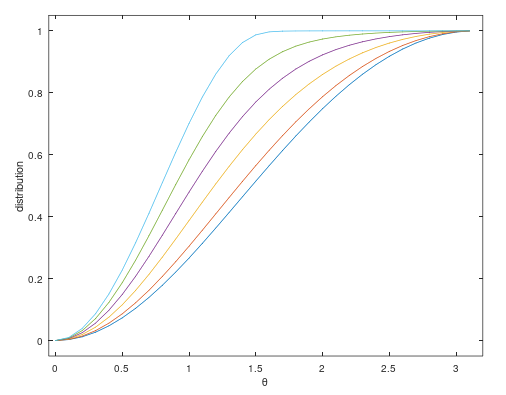
\includegraphics[width=10cm]{chapter_04_paragraph_16_exercice_2a}
		\caption{Exemples de distribution pour diff\'erentes valeurs de $\frac{V}{v_{0}}$, de 0.1 à 0.99, par int\'egration de l'\'equation (\ref{EQ:16_EX2A})}\label{FIG:4_16_EX2A}
	\end{center}
\end{figure}

\subsubsection{$v_{0} < V$}

Dans ce cas, la m\^eme s\'equence calculatoire am\`ene \`a \'ecrire pour $\theta \in [0;\theta_{max}]$ :
\be
	\begin{Bmatrix}\dfrac{\mathrm{d}\omega_{0}}{4\pi}\end{Bmatrix}_{2} = \dfrac{1}{2}\sin\theta\left[2\dfrac{V}{v_{0}}\cos\theta - \dfrac{1 + \dfrac{V^{2}}{v_{0}^{2}}\cos(2\theta)}{\sqrt{1 - \dfrac{V^{2}}{v_{0}^{2}}\sin^{2}\theta}}\right]\mathrm{d}\theta
\ee
sachant qu'il faut prendre cette fois-ci dans l'\'equation (\ref{EQ:16_6}) les deux solutions, celles avec le signe - et celle avec le signe +, d\'eduite pr\'ec\`edemment. Ainsi la distribution totale pour $v_{0} < V$ s'obtient en faisant :
\be
	\begin{Bmatrix}\dfrac{\mathrm{d}\omega_{0}}{4\pi}\end{Bmatrix}_{1} - \begin{Bmatrix}\dfrac{\mathrm{d}\omega_{0}}{4\pi}\end{Bmatrix}_{2} = \dfrac{1 + \dfrac{V^{2}}{v_{0}^{2}}\cos(2\theta)}{\sqrt{1 - \dfrac{V^{2}}{v_{0}^{2}}\sin^{2}\theta}}\sin\theta\mathrm{d}\theta\label{EQ:16_EX2B}
\ee

\begin{figure}[htb!]
	\begin{center}
		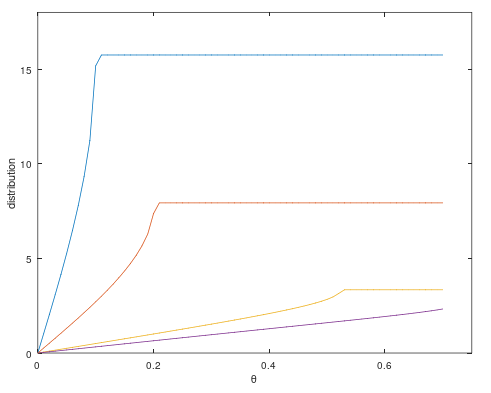
\includegraphics[width=10cm]{chapter_04_paragraph_16_exercice_2b}
		\caption{Exemples de distribution pour diff\'erentes valeurs de $\frac{V}{v_{0}}$, de 1.5 à 10, par int\'egration de l'\'equation (\ref{EQ:16_EX2B})}\label{FIG:4_16_EX2B}
	\end{center}
\end{figure}

\subsection{Intervalles angulaires dans <<~l~>>}

Dans le r\'ef\'erentiel <<~l~>>, d\'eterminons l'angle $\theta$ d\'efini comme la somme $\theta_{1} + \theta_{2}$ :
\bea
	\tan\theta & = & \tan(\theta_{1} + \theta_{2}) = \dfrac{\tan\theta_{1} + \tan\theta_{2}}{1 - \tan\theta_{1}\tan\theta_{2}} \nonumber \\
	& = & \dfrac{\dfrac{v_{10}\sin\theta_{10}}{V + v_{10}\cos\theta_{10}} + \dfrac{v_{20}\sin\theta_{20}}{V + v_{20}\cos\theta_{20}}}{1 - \dfrac{v_{10}\sin\theta_{10}}{V + v_{10}\cos\theta_{10}}\dfrac{v_{20}\sin\theta_{20}}{V + v_{20}\cos\theta_{20}}} \nonumber \\
\eea
or $\theta_{20} = \pi - \theta_{10}$, donc :
\bea
	\tan\theta & = & \dfrac{\dfrac{v_{10}\sin\theta_{10}}{V + v_{10}\cos\theta_{10}} + \dfrac{v_{20}\sin\theta_{10}}{V - v_{20}\cos\theta_{10}}}{1 - \dfrac{v_{10}\sin\theta_{10}}{V + v_{10}\cos\theta_{10}}\dfrac{v_{20}\sin\theta_{10}}{V - v_{20}\cos\theta_{10}}} \nonumber \\
	& = & \dfrac{v_{10}\sin\theta_{10}(V - v_{20}\cos\theta_{10}) + v_{20}\sin\theta_{10}(v_{10}\cos\theta_{10} + V)}{(V + v_{10}\cos\theta_{10})(V - v_{20}\cos\theta_{10}) - v_{10}v_{20}\sin^{2}\theta_{10}} \nonumber \\
	& = & \dfrac{v_{10}V\sin\theta_{10} - v_{10}v_{20}\cos\theta_{10}\sin\theta_{10} + v_{10}v_{20}\cos\theta_{10}\sin\theta_{10} + v_{20}V\sin\theta_{10}}{v_{10}V\cos\theta_{10} - v_{10}v_{20}\cos^{2}\theta_{10} + V^{2} - v_{20}V\cos\theta_{10} - v_{10}v_{20}\sin^{2}\theta_{10}} \nonumber \\
	& = & \dfrac{(v_{10} + v_{20})V\sin\theta_{10}}{V^{2} - v_{10}v_{20} + (v_{10} - v_{20})V\cos\theta_{10}}
\eea

\section{Chocs \'elastiques de deux particules}

Dans le r\'ef\'erentiel <<~l~>>, exprimons les vitesses apr\`es le choc $v'_{1}$ et $v'_{2}$ en fonction de l'angle de d\'eviation sous lequel elles s'\'ecartent, sachant qu'avant le choc $v_{2} = 0$ et donc $v_{1} = v$.

Puisque la grandeur $2OB$ est un diam\`etre du cercle de rayon $mv$, nous avons $p'_{2} = 2OB\cos\theta_{2}$, donc :
\be
	v'_{2} = \dfrac{2OB}{m_{2}}\cos\theta_{2} = \dfrac{2mv}{m_{2}}\cos\theta_{2}
\ee
avec $m$ la masse r\'eduite du syst\`eme compos\'e des deux particules.

Ensuite, nous utilisons la formule d'Al-Kashi dans le triangle form\'e des points $A$, $O$ et $C$, voir la figure (\ref{FIG:4_16}) pour faire intervenir l'angle $\theta_{1}$ tel que :
\bea
	OC^{2} & = & AO^{2} + {p'}_{1}^{2} - 2 AOp'_{1}\cos\theta_{1} \nonumber \\
	m^{2}v^{2} & = & \dfrac{m_{1}^{2}}{m_{2}^{2}}OB^{2} + m_{1}^{2}{v'}_{1}^{2} - 2\dfrac{m_{1}^{2}}{m_{2}}OBv'_{1}\cos\theta_{1} \nonumber \\
	\left(1 - \dfrac{m_{1}^{2}}{m_{2}^{2}}\right)m^{2}v^{2} & = & m_{1}^{2}{v'}_{1}^{2} - 2\dfrac{m_{1}^{2}}{m_{2}}mvv'_{1}\cos\theta_{1} \nonumber \\
	\dfrac{(m_{2} + m_{1})(m_{2} - m_{1})}{m_{2}^{2}}m^{2} & = & m_{1}^{2}\dfrac{v'_{1}}{v}^{2} - 2\dfrac{m_{1}^{2}}{m_{2}}m\dfrac{v'_{1}}{v}\cos\theta_{1} \nonumber \\
	\dfrac{(m_{2} + m_{1})(m_{2} - m_{1})m_{1}^{2}m_{2}^{2}}{m_{2}^{2}(m_{1} + m_{2})} & = & m_{1}^{2}\dfrac{v'_{1}}{v}^{2} - 2\dfrac{m_{1}^{2}}{m_{2}}m\dfrac{v'_{1}}{v}\cos\theta_{1} \nonumber \\
	0 & = & \left(\dfrac{v'_{1}}{v}\right)^{2} - 2\dfrac{m}{m_{2}}\dfrac{v'_{1}}{v}\cos\theta_{1} + \dfrac{m_{1} - m_{2}}{m_{1} + m_{2}}
\eea

Il s'agit d'une \'equation du second degr\'e en $v'_{1}/v$ dont les solutions sont :
\bea
	\dfrac{v'_{1}}{v} & = & \dfrac{1}{2}\left(\dfrac{2m_{1}m_{2}}{m_{2}(m_{1} + m_{2})}\cos\theta_{1} \pm \sqrt{\dfrac{4m_{1}^{2}m_{2}^{2}}{m_{2}^{2}(m_{1} + m_{2})^{2}}\cos^{2}\theta_{1} - \dfrac{4(m_{1} - m_{2})}{m_{2}(m_{1} + m_{2})}}\right) \nonumber \\
	& = & \dfrac{m_{1}}{m_{1} + m_{2}}\cos\theta_{1} \pm \sqrt{\dfrac{m_{1}^{2}}{(m_{1} + m_{2})^{2}}\cos^{2}\theta_{1} - \dfrac{m_{1}^{2} - m_{2}^{2}}{(m_{1} + m_{2})^{2}}} \nonumber \\
	& = & \dfrac{m_{1}}{m_{1} + m_{2}}\cos\theta_{1} \pm \dfrac{1}{m_{1} + m_{2}}\sqrt{m_{2}^{2} + (\cos^{2}\theta_{1} - 1)m_{1}^{2}} \nonumber \\
	& = & \dfrac{m_{1}}{m_{1} + m_{2}}\cos\theta_{1} \pm \dfrac{m_{2}}{m_{1} + m_{2}}\sqrt{1 + \dfrac{m_{1}^{2}}{m_{2}^{2}}\sin^{2}\theta_{1}}
\eea
De mani\`ere \'equivalente \`a l'\'equation (\ref{EQ:16_6}), pour $m_{1} > m_{2}$, la solution est univoque avec le signe $+$ alors que pour $m_{1} < m_{2}$, les deux solutions sont admises. La repr\'esentation de ces solutions est \'egalement similaire \`a ce qui est repr\'esent\'e sur les figures (\ref{FIG:4_14A}) et (\ref{FIG:4_14B}).

\section{Diffusion des particules}

\subsection{Diffusion par une bille solide}\label{PAR:18EX}

\begin{figure}[htb!]
	\begin{center}
		\begin{picture}(300,200)(0,0)
			%circle
			\linethickness{0.05mm}
			\put(50,50){\circle{100}}
			%dashed lines
			\linethickness{0.05mm}
			\multiput(50,50)(10,0){25}{\line(1,0){8}}
			\put(65,75){$a$}
			\multiput(50,50)(10,10){10}{\line(1,1){8}}
			%angles
			\qbezier(60,50)(60,55)(55,55)
			\put(60,57){$\varphi_{0}$}
			%vectors
			\put(150,73){\vector(0,1){12}}
			\put(150,63){\vector(0,-1){13}}
			\put(147,66){$\rho$}
			%trajectories
			\linethickness{0.5mm}
			\put(85,85){\line(1,0){220}}
			\put(85,85){\line(2,5){40}}
		\end{picture}
		\caption{Diffusion par une bille solide de rayon $a$}\label{FIG:4_18_EX1}
	\end{center}
\end{figure}

L'objectif est de calculer la section efficace pour la diffusion de particules par une bille de rayon $a$ parfatiement solide, i.e. $U(r>a) = 0$ et $U(r<a) = \infty$. La figure (\ref{FIG:4_18_EX1}) illustre la trajectoire, \`a savoir que les particules incidentes se meuvent librement avant et apr\`es le choc, qui se compose de deux droites. D'apr\`es la m\^eme figure, nous pouvons \'etablir que :
\bea
	\rho & = & a\sin\varphi_{0} = a\sin\left(\dfrac{\pi - \xi}{2}\right) = a\left(\cos\dfrac{\pi}{2}\sin\dfrac{-\xi}{2} + \sin\dfrac{\pi}{2}\cos\dfrac{-\xi}{2}\right) \nonumber \\
	& = & a\cos\dfrac{\xi}{2}
\eea
En reportant dans l'\'equation (\ref{EQ:18_7}), cela donne :
\be
	\mathrm{d}\sigma = 2\pi a\cos\dfrac{\xi}{2}\lvert -\dfrac{a}{2}\sin\dfrac{\xi}{2} \rvert \mathrm{d}\xi = \pi a^{2}\cos\dfrac{\xi}{2}\sin\dfrac{\xi}{2}\mathrm{d}\xi
\ee
or $\sin\xi = \sin(\frac{\xi}{2} + \frac{\xi}{2}) = 2\cos\frac{\xi}{2}\sin\frac{\xi}{2}$, donc :
\be
	\mathrm{d}\sigma = \dfrac{\pi a^{2}}{2}\sin\xi\mathrm{d}\xi
\ee
et puisque l'angle solide se d\'efinit pour un anneau comme $\mathrm{d}\omega = 2\pi\sin\xi\mathrm{d}\xi$, donc :
\be
	\mathrm{d}\sigma = \dfrac{a^{2}}{4}\mathrm{d}\omega
\ee
Dans le r\'ef\'erentiel <<~c~>>, la distribution est donc isotrope, i.e. ne d\'epend pas de l'angle de d\'eviation, puisque :
\be
	\sigma = \int_{0}^{4\pi}\dfrac{a^{2}}{4}\mathrm{d}\omega = \pi a^{2}
\ee
et la section efficace est \'egale \`a la section de la bille et assez logiquement, une particule pour \^etre diffus\'ee doit avoir une distance de vis\'ee inf\'erieure au rayon\footnote{Les particules incdents sont consid\'er\'ees comme ponctuelles.} de la bille $a$. Pour d\'eterminer la section efficace $\mathrm{d}\sigma$ dans le r\'ef\'erentiel <<~l~>>, nous pouvons repartir des \'equations (\ref{EQ:17_4}) o\`u $m_{1}$ est la masse de la particule incidente et $m_{2}$ celle de la bille. Nous avons vu plus haut que :
\be
	\mathrm{d}\sigma = \dfrac{\pi a^{2}}{2}\sin\xi\mathrm{d}\xi = -\dfrac{\pi a^{2}}{2}\mathrm{d}(\cos\xi)
\ee
La quantit\'e $\cos\xi$ est reprise de l'\'equation (\ref{EQ:18_9}) et il y a trois cas diiff\'erents.

\subsubsection{$m_{1} < m_{2}$}

Dans ce cas, $\cos\xi$ s'\'ecrit :
\be
	\cos\xi = -\dfrac{m_{1}}{m_{2}}\sin^{2}\theta_{1} + \cos\theta_{1}\sqrt{1 - \dfrac{m_{1}^{2}}{m_{2}^{2}}\sin^{2}\theta_{1}}
\ee
aussi :
\bea
	\mathrm{d}(\cos\xi) & = & -2\dfrac{m_{1}}{m_{2}}\cos\theta_{1}\sin\theta_{1}\mathrm{d}\theta_{1} - \sin\theta_{1}\mathrm{d}\theta_{1}\sqrt{1 - \dfrac{m_{1}^{2}}{m_{2}^{2}}\sin^{2}\theta_{1}} + \dfrac{1}{2}\cos\theta_{1}\dfrac{-2\dfrac{m_{1}^{2}}{m_{2}^{2}}\cos\theta_{1}\sin\theta_{1}\mathrm{d}\theta_{1}}{\sqrt{1 - \dfrac{m_{1}^{2}}{m_{2}^{2}}\sin^{2}\theta_{1}}} \nonumber \\
	& = & -\sin\theta_{1}\mathrm{d}\theta_{1}\left(2\dfrac{m_{1}}{m_{2}}\cos\theta_{1} + \sqrt{1 - \dfrac{m_{1}^{2}}{m_{2}^{2}}\sin^{2}\theta_{1}} + \dfrac{\dfrac{m_{1}^{2}}{m_{2}^{2}}\cos^{2}\theta_{1}}{\sqrt{1 - \dfrac{m_{1}^{2}}{m_{2}^{2}}\sin^{2}\theta_{1}}}\right) \nonumber \\
	& = & -\sin\theta_{1}\mathrm{d}\theta_{1}\left(2\dfrac{m_{1}}{m_{2}}\cos\theta_{1} + \dfrac{1}{\sqrt{1 - \dfrac{m_{1}^{2}}{m_{2}^{2}}\sin^{2}\theta_{1}}}\left(1 - \dfrac{m_{1}^{2}}{m_{2}^{2}}\sin^{2}\theta_{1} + \dfrac{m_{1}^{2}}{m_{2}^{2}}\cos^{2}\theta_{1}\right)\right) \nonumber \\
	& = & -\sin\theta_{1}\mathrm{d}\theta_{1}\left(2\dfrac{m_{1}}{m_{2}}\cos\theta_{1} + \dfrac{1}{\sqrt{1 - \dfrac{m_{1}^{2}}{m_{2}^{2}}\sin^{2}\theta_{1}}}\left(1 + \dfrac{m_{1}^{2}}{m_{2}^{2}}(\cos^{2}\theta_{1} - \sin^{2}\theta_{1})\right)\right) \nonumber \\
	& = & -\sin\theta_{1}\mathrm{d}\theta_{1}\left(2\dfrac{m_{1}}{m_{2}}\cos\theta_{1} + \dfrac{1}{\sqrt{1 - \dfrac{m_{1}^{2}}{m_{2}^{2}}\sin^{2}\theta_{1}}}\left(1 + \dfrac{m_{1}^{2}}{m_{2}^{2}}\cos(2\theta_{1})\right)\right)
\eea
donc :
\be
	\mathrm{d}\sigma_{1} = \dfrac{\pi a^{2}}{2}\left(2\dfrac{m_{1}}{m_{2}}\cos\theta_{1} + \dfrac{1 + \dfrac{m_{1}^{2}}{m_{2}^{2}}\cos(2\theta_{1})}{\sqrt{1 - \dfrac{m_{1}^{2}}{m_{2}^{2}}\sin^{2}\theta_{1}}}\right)\sin\theta_{1}\mathrm{d}\theta_{1}
\ee
et puisque $\mathrm{d}\omega_{1} = 2\pi\sin\theta_{1}\mathrm{d}\theta_{1}$, nous avons finalement :
\be
	\mathrm{d}\sigma_{1+} = \dfrac{a^{2}}{4}\left(2\dfrac{m_{1}}{m_{2}}\cos\theta_{1} + \dfrac{1 + \dfrac{m_{1}^{2}}{m_{2}^{2}}\cos(2\theta_{1})}{\sqrt{1 - \dfrac{m_{1}^{2}}{m_{2}^{2}}\sin^{2}\theta_{1}}}\right)\mathrm{d}\omega_{1}
\ee

\subsubsection{$m_{1} > m_{2}$}

Dans ce cas, il nous faut prendre les deux solutions de l'\'equation (\ref{EQ:18_9}). Nous pouvons reprendre celle avec le signe $+$ de la pr\'ec\'edente section et calculons la section efficace pour la seconde solution de $\cos\xi$, celle qui s'\'ecrit ainsi :
\be
	\cos\xi = -\dfrac{m_{1}}{m_{2}}\sin^{2}\theta_{1} - \cos\theta_{1}\sqrt{1 - \dfrac{m_{1}^{2}}{m_{2}^{2}}\sin^{2}\theta_{1}}
\ee
En appliquant les m\^emes calculs, nous arrivons \`a :
\be
	\mathrm{d}\sigma_{1-} = \dfrac{a^{2}}{4}\left(2\dfrac{m_{1}}{m_{2}}\cos\theta_{1} - \dfrac{1 + \dfrac{m_{1}^{2}}{m_{2}^{2}}\cos(2\theta_{1})}{\sqrt{1 - \dfrac{m_{1}^{2}}{m_{2}^{2}}\sin^{2}\theta_{1}}}\right)\mathrm{d}\omega_{1}
\ee
En d\'efinitive, nous obtenons :
\be
	\mathrm{d}\sigma_{1} = \mathrm{d}\sigma_{1+} - \mathrm{d}\sigma_{1-} = \dfrac{a^{2}}{2}\dfrac{1 + \dfrac{m_{1}^{2}}{m_{2}^{2}}\cos(2\theta_{1})}{\sqrt{1 - \dfrac{m_{1}^{2}}{m_{2}^{2}}\sin^{2}\theta_{1}}}\mathrm{d}\omega_{1}
\ee

\subsubsection{$m_{1} = m_{2}$}

Dans ce cas pr\'ecis, nous en d\'eduisons :
\bea
	\mathrm{d}\sigma_{1} & = & \dfrac{a^{2}}{2}\dfrac{1 + \cos(2\theta_{1})}{\sqrt{1 - \sin^{2}\theta_{1}}}\mathrm{d}\omega_{1} = \dfrac{a^{2}}{2}\dfrac{1 + \cos^{2}\theta_{1} - \sin^{2}\theta_{1}}{\lvert \cos\theta_{1} \rvert}\mathrm{d}\omega_{1} = \dfrac{a^{2}}{2}\dfrac{1 + \cos^{2}\theta_{1} - 1 + \cos^{2}\theta_{1}}{\lvert \cos\theta_{1} \rvert}\mathrm{d}\omega_{1} \nonumber \\
	& = & a^{2}\lvert \cos\theta_{1} \rvert\mathrm{d}\omega_{1}
\eea
$\cos\theta_{1}$ n'est pas forc\`ement positif, aussi il nous faut utiliser sa valeur absolue car la section efficace reste une surface et donc a une valeur positive.

Enfin, dans le cas o\`u initialement, i.e. avant le choc, la bille de masse $m_{2}$ est immobile, comme $\xi = \pi - 2\theta_{2}$, alors :
\bea
	\mathrm{d}\sigma_{2} & = & \dfrac{\pi a^{2}}{2}\sin(\pi - 2\theta_{2})\mathrm{d}(\pi - 2\theta_{2}) = \dfrac{\pi a^{2}}{2}\sin(2\theta_{2})\cdot -2\mathrm{d}(\theta_{2}) = -\pi a^{2}\sin(2\theta_{2})\mathrm{d}(\theta_{2}) \nonumber \\
	& = & -2\pi a^{2}\cos\theta_{2}\sin\theta_{2}\mathrm{d}\theta_{2}
\eea
or comme $\mathrm{d}\omega_{2} = 2\pi\sin\theta_{2}\mathrm{d}\theta_{2}$ et $\mathrm{d}\sigma_{2} > 0$, nous avons finalement :
\be
	\mathrm{d}\sigma_{2} = a^{2}\lvert \cos\theta_{2} \rvert\mathrm{d}\omega_{2}
\ee

\subsection{\'Energie perdue}

Il s'agit de calculer la section efficace de diffusion en fonction de l'\'energie perdue $\epsilon$ par les particules diffus\'ees de masse $m_{1}$ dans le m\^eme cas que dans le paragraphe (\ref{PAR:18EX}). La loi de conservation de l'\'energie du syst\`eme ferm\'e implique que $\epsilon$ vaut exactement l'\'energie gagn\'ee par $m_{2}$. Cette derni\`ere est l'\'energie cin\'etique gagn\'ee par $m_{2}$ apr\`es le choc car dans le cas pr\'esent, avant le choc, $v_{2} = 0$. L'utilisation de l'\'equation (\ref{EQ:17_5B}) permet d'\'ecrire :
\be
	v'_{2} = \dfrac{2m_{1}v}{m_{1} + m_{2}}\sin\left(\dfrac{\xi}{2}\right) = \dfrac{2m_{1}v_{\infty}}{m_{1} + m_{2}}\sin\left(\dfrac{\xi}{2}\right)
\ee
car $v = v_{1} = v_{\infty}$ puisque $v_{1}$ est la vitesse avant le choc de la particule de masse $m_{1}$. Donc l'\'energie de la particule de masse $m_{2}$ apr\`es le choc vaut :
\bea
	E'_{2} & = & \dfrac{m_{2}}{2}{v'}_{2}^{2} = \dfrac{m_{2}}{2}\dfrac{m_{1}^{2}v_{\infty}^{2}}{(m_{1} + m_{2})^{2}}\sin^{2}\left(\dfrac{\xi}{2}\right) \nonumber \\
	\Leftrightarrow \epsilon & = & \dfrac{2m_{1}^{2}m_{2}}{(m_{1} + m_{2})^{2}}v_{\infty}^{2}\sin^{2}\left(\dfrac{\xi}{2}\right)
\eea
Par d\'efinition, $\sin^{2}(\frac{\xi}{2}) \leq 1$, nous pouvons donc en d\'eduire que l'\'energie perdue maximale $\epsilon_{max}$ vaut pr\'ecis\`ement :
\be
	\epsilon_{max} = \dfrac{2m_{1}^{2}m_{2}}{(m_{1} + m_{2})^{2}}v_{\infty}^{2}
\ee
telle que :
\be
	\epsilon = \epsilon_{max}\sin^{2}\left(\dfrac{\xi}{2}\right)
\ee
En d\'erivant, nous obtenons :
\be
	\mathrm{d}\epsilon = \epsilon_{max}\sin\left(\dfrac{\xi}{2}\right)\cos\left(\dfrac{\xi}{2}\right)\mathrm{d}\xi = \dfrac{1}{2}\epsilon_{max}\sin\xi\mathrm{d}\xi
\ee
car $\sin\xi = 2\sin(\frac{\xi}{2})\cos(\frac{\xi}{2})$. Nous savons que :
\be
	\mathrm{d}\sigma = \dfrac{\pi a^{2}}{2}\sin\xi\mathrm{d}\xi
\ee
donc, finalement :
\be
	\mathrm{d}\sigma = \dfrac{\pi a^{2}}{\epsilon_{max}}\mathrm{d}\epsilon
\ee
et la distribution des particules diffus\'ees est homog\`ene par rapport \`a $\epsilon$ qui est l'\'energie perdue par celles-ci.

\subsection{Cas d'un champ $\propto r^{-n}$}

Nous allons d\'eterminer la relation entre la section efficace et $v_{\infty}$ dans le cadre o\`u l'\'energie potentielle est proportionnelle \`a $r^{-n}$. Dans le cadre d'une \'energie potentielle homog\`ene d'ordre $k = -n$, les relations (\ref{EQ:10_3}) donnent en particulier :
\be
	\dfrac{v'}{v} = \left(\dfrac{l'}{l}\right)^{-\dfrac{n}{2}}
\ee
qui exprime la relation entre la vitesse et la longueur pour deux trajectoires diff\'erentes. Nous pouvons ainsi \'ecrire que $\rho\propto v^{-\frac{2}{n}}$ pour des trajectoires semblables. Ceci peut \^etre exprimer telle que $\rho = v_{\infty}^{-\frac{2}{n}}f(\xi)$ car pour chaque trajectoire semblable, l'angle de d\'eviation est identique. En substituant dans l'\'equation (\ref{EQ:18_6}), nous avons :
\be
	\mathrm{d}\sigma = 2\pi\rho\mathrm{d}\rho = 2\pi v_{\infty}^{-\frac{2}{n}}f(\xi)\cdot v_{\infty}^{-\frac{2}{n}}f'(\xi)\mathrm{d}\xi = 2\pi v_{\infty}^{-\frac{4}{n}}f(\xi)f'(\xi)\mathrm{d}\xi
\ee
or :
\be
	\mathrm{d}\omega = 2\pi\sin\xi\mathrm{d}\xi \Rightarrow \mathrm{d}\xi = \dfrac{\mathrm{d}\omega}{2\pi\sin\xi}
\ee
soit :
\be
	\mathrm{d}\sigma = 2\pi v_{\infty}^{-\frac{4}{n}}\dfrac{f(\xi)f'(\xi)}{2\pi\sin\xi}\mathrm{d}\omega = v_{\infty}^{-\frac{4}{n}}\dfrac{f(\xi)f'(\xi)}{\sin\xi}\mathrm{d}\omega \propto v_{\infty}^{-\frac{4}{n}}\mathrm{d}\omega
\ee

\subsection{Cas d'un champ $U = -\alpha / r^{2}$}

Pour d\'eterminer la section efficace pour une <<~chute~>> de particules au centre d'un champ tel que $U = -\alpha / r^{2}$, nous pouvons reprendre la d\'emonstration r\'ealis\'ee à l'\'equation {\ref{EQ:14_11}) et puisque $n = 2$, les particules incidentes de masse $m$ <<~tombent~>> si et seulement si $\alpha > \frac{M^{2}}{2m}$. En utilisant la d\'efinition (\ref{EQ:18_3}) du moment cin\'etique telle $M = m\rho v_{\infty}$, nous avons :
\be
	\alpha > \dfrac{M^{2}}{2m} \Leftrightarrow \alpha > \dfrac{m^{2}\rho^{2}v_{\infty}^{2}}{2m} \Leftrightarrow \rho^{2} < \dfrac{2\alpha}{mv_{\infty}^{2}}
\ee
Comme cela implique que la distance de vis\'ee maximale vaut exactement $\rho_{max} = \sqrt{\frac{2\alpha}{mv_{\infty}^{2}}}$ et cela donne de facto la section efficace de chute :
\be
	\sigma = \pi\rho_{max}^{2} = \dfrac{2\pi\alpha}{mv_{\infty}^{2}}
\ee

\subsection{Cas d'un champ $U = -\alpha / r^{n}$}

\begin{figure}[htb!]
	\begin{center}
		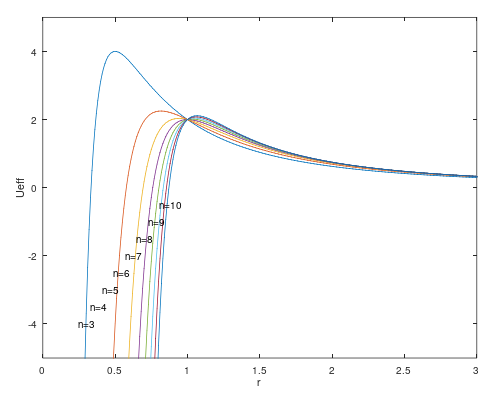
\includegraphics[width=10cm]{chapter_04_paragraph_18_exercice_5}
		\caption{\'Energie potentielle efficace pour $m\rho^{2}v_{\infty}^{2} = 6$ et $\alpha = 1$.}\label{FIG:4_18_5}
	\end{center}
\end{figure}

Ici, nous consid\'erons que $n > 2$ et $\alpha > 0$. En reprenant l'\'equation (\ref{EQ:14_8}) et puisque nous \'etudions un champ central, l'\'energie potentielle efficace s'\'ecrit :
\be
	U_{eff}(r) = U(r) + \dfrac{M^{2}}{2mr^{2}} = \dfrac{m\rho^{2}v_{\infty}^{2}}{2r^{2}} - \dfrac{\alpha}{r^{n}}
\ee
et dont une illustration est pr\'esente sur la figure (\ref{FIG:4_18_5}). Dans ce cas, les particules incidentes <<~tombent~>> au centre si et seulement si leur \'energie $E$ est sup\'erieure \`a $U_{0}$ qui correspond à la valeur maximale de l'\'energie potentielle efficace $U_{eff}(r)$. La figure (\ref{FIG:4_18_5}) montre que trouver un extremum \`a $U_{eff}(r)$ revient \`a trouver son maximum, soit r\'esoudre l'\'equation :
\bea
	\dfrac{\mathrm{d}U_{eff}(r)}{\mathrm{d}r} & = & 0 \Leftrightarrow -\dfrac{m\rho^{2}v_{\infty}^{2}}{r^{3}} + \dfrac{\alpha n}{r^{n + 1}} = 0 \Leftrightarrow m\rho^{2}v_{\infty}^{2} = \dfrac{\alpha n}{r_{0}^{n - 2}} \nonumber \\
	r_{0} & = & \left(\dfrac{n\alpha}{m\rho^{2}v_{\infty}^{2}}\right)^{\dfrac{1}{n - 2}}
\eea
ce qui permet de calculer la valeur maximale de l'\'energie potentielle efficace :
\bea
	U_{eff\, max} & = & U(r_{0}) = \dfrac{m\rho^{2}v_{\infty}^{2}}{2\left(\dfrac{n\alpha}{m\rho^{2}v_{\infty}^{2}}\right)^{\frac{2}{n - 2}}} - \dfrac{\alpha}{\left(\dfrac{n\alpha}{m\rho^{2}v_{\infty}^{2}}\right)^{\frac{n}{n - 2}}} \nonumber \\
	& = & \dfrac{m\rho^{2}v_{\infty}^{2}}{2}\left(\dfrac{m\rho^{2}v_{\infty}^{2}}{n\alpha}\right)^{\frac{2}{n - 2}} - \alpha\left(\dfrac{m\rho^{2}v_{\infty}^{2}}{n\alpha}\right)^{\frac{n}{n - 2}} \nonumber \\
	& = & \left(\dfrac{m\rho^{2}v_{\infty}^{2}}{n\alpha}\right)^{\frac{n}{n - 2}}\left(-\alpha + \dfrac{m\rho^{2}v_{\infty}^{2}}{2}\left(\dfrac{m\rho^{2}v_{\infty}^{2}}{n\alpha}\right)^{\frac{2 - n}{n - 2}}\right) \nonumber \\
	& = & \left(\dfrac{m\rho^{2}v_{\infty}^{2}}{n\alpha}\right)^{\frac{n}{n - 2}}\left(-\alpha + \dfrac{m\rho^{2}v_{\infty}^{2}}{2}\dfrac{n\alpha}{m\rho^{2}v_{\infty}^{2}}\right) = \dfrac{n - 2}{2}\alpha\left(\dfrac{m\rho^{2}v_{\infty}^{2}}{n\alpha}\right)^{\frac{n}{n - 2}} \nonumber \\
\eea
La distance de vis\'ee maximale $\rho_{max}$ se d\'efinit comme la distance de vis\'ee au-del\`a de laquelle l'\'energie de la particule incidente est sup\'erieure \`a $U_{eff\, max}$. Par d\'efinition, les particules incidentes ont pour \'energie $E = \frac{m}{2}v_{\infty}^{2}$. En posant $E = U_{eff\, max}$, nous obtenons :
\bea
	mv_{\infty}^{2} & = & (n - 2)\alpha\left(\dfrac{m\rho_{max}^{2}v_{\infty}^{2}}{n\alpha}\right)^{\frac{n}{n - 2}} \Leftrightarrow \rho_{max}^{2} = \left(\dfrac{mv_{\infty}^{2}}{(n - 2)\alpha}\right)^{\frac{n - 2}{n}}\dfrac{n\alpha}{mv_{\infty}^{2}} \nonumber \\
	\Leftrightarrow \rho_{max}^{2} & = & n(n - 2)^{\frac{2 - n}{n}}\left(\dfrac{mv_{\infty}^{2}}{\alpha}\right)^{\frac{n - 2}{n} - 1} = n(n - 2)^{\dfrac{2 - n}{n}}\left(\dfrac{\alpha}{mv_{\infty}^{2}}\right)^{\frac{n}{2}}
\eea
et la section efficace de chute s'\'ecrit :
\be
	\sigma = \pi\rho_{max}^{2} = \pi n(n - 2)^{\frac{2 - n}{n}}\left(\dfrac{\alpha}{mv_{\infty}^{2}}\right)^{\frac{n}{2}}
\ee

\subsection{Cas d'un champ suivant la loi de Newton}

\subsection{M\'ethode d'inversion de Firsov}

Oleg Firsov, 1953 cit\'e dans un article de 1971\footnote{Uniqueness of the Firsov Inversion Method and Focusing Potentials, Yu.N. Demkov, V.N. Ostrovskii, et N.B. Berezina}